
\appendix

% 5 lines below for creating appendix table of content
\renewcommand \thepart{}
\renewcommand \partname{}
\addcontentsline{toc}{section}{Appendix} % Add the appendix text to the document TOC
\part{Appendix} % Start the appendix part
\parttoc % Insert the appendix TOC


\clearpage
\section{Pseudocode for the extended CrossWalk algorithm}


\begin{algorithm}
\caption{CrossWalk algorithm}
\label{alg:crosswalk}
\begin{algorithmic}[1]
\Require Graph $G = (V, E, w)$, edge weights $w_{uv}>0$ for all $(v, u) \in E$, parameters $\alpha \in (0,1), p>0$.
\Ensure Updated weights $w'_{vu}$ for all $(v, u) \in E$.
\For{$v \in V$} \Comment{Estimate colorfulness of nodes}
    \State Run $r$ random walks $\mathcal{W}_v^j$, $j \in \{ 1, \dots, r \}$, rooted at $v$.
    \State $m(v) = \left( \sum_{j = 1}^r \sum_{u \in \mathcal{W}_v^j} \mathbb{I}[c(v) \neq c(u)] \right) / rd$ \Comment{[\autoref{eq:colorfulness}]}
\EndFor
\For{$v \in V$} \Comment{Iterate through all nodes}
    \State $R_v = \{ c(u) \ | \ u \in \mathcal{N}(v) \} \setminus c(v)$
    \For{$c \in \{ c(u) \ | \ u \in \mathcal{N}(v) \}$} \Comment{Iterate through all colors neighboring $v$}
        \State $N_v^{c} = \{ u \in \mathcal{N}(v) \ | \ c(u) = c \}$
        \For{$u \in N_v^{c}$} \Comment{Iterate through $v$'s neighbors of color $c$}
            \If{$\exists z \in N_v^c : m(z) > 0$}
                \State $n = \left( w_{vu} m(u)^p \right) / \left( \sum_{z \in N_v^c} w_{vz} m(z)^p \right)$ \Comment{[\autoref{eq:crosswalk:norm1}]}
            \Else
                \State $n = w_{vu} / \sum_{z \in N_v^c} w_{vz}$ \Comment{[\autoref{eq:crosswalk:norm2}]}
            \EndIf
            \If{$c = c(v)$} \Comment{Reweight edges towards same group}
                \If{$\exists z \in \mathcal{N}(v) : c(z) \neq c(v)$}
                % \If{$\mathcal{N}(v) \neq N_v^c$}
                    \State $w_{vu}' = (1-\alpha) n$ \Comment{[\autoref{eq:crosswalk:base1}]}
                \Else
                    \State $w_{vu}' = n$ \Comment{[\autoref{eq:crosswalk:add1}]}
                \EndIf
            \Else \Comment{Reweight edges connecting different groups}
                \If{$\exists z \in \mathcal{N}(v) : c(z) = c(v)$}
                    \State $w_{vu}' = \alpha n / |R_v|$ \Comment{[\autoref{eq:crosswalk:base2}]}
                \Else
                    \State $w_{vu}' = n / |R_v|$ \Comment{[\autoref{eq:crosswalk:add2}]}
                \EndIf
            \EndIf
        \EndFor
    \EndFor
\EndFor
\end{algorithmic}
\end{algorithm}

\clearpage
\section{Proof of Theorem 1}
\label{sec:proof}
\begin{proof}
For any node $v \in V$, three situations may occur. The node $v$ may have (a) at least one same-colored and one differently-colored neighbor, (b) only neighbors of the same color, or (c) only neighbors of a different color. The possibility of nodes without outgoing edges is excluded by requirement. Further, we assume that for every neighboring group of $v$, there exists a neighboring node with a non-zero colorfulness, i.e. $n_{vu} = \frac{w_{vu} m(u)^p}{\sum_{z \in N_v^{c(u)}} w_{vz} m(z)^p}$ (\autoref{eq:crosswalk:norm1}). For the other cases handled by (\autoref{eq:crosswalk:norm2}), the proof follows in the exact same manner.
\begin{enumerate}
    \item[(a)] If node $v$ has at least one same-colored and one differently-colored neighbor, i.e. $\mathcal{N}(v) \neq N_v^{c(v)} \wedge \mathcal{N}(v) \neq \left( \bigcup_{c \in R_v} N_v^{c} \right)$, then $w_{vu}' = (1-\alpha) n_{vu}$ for $u \in N_v^{c(v)}$ (\autoref{eq:crosswalk:base1}) and $w_{vu}' = \frac{\alpha}{|R_v|} n_{vu}$ for $u \in N_v^c$, $c \in R_v$ (\autoref{eq:crosswalk:base2})
    \begin{align*}
         \Rightarrow \sum_{u \in \mathcal{N}(v)} w_{vu}' &= \sum_{u \in N_v^{c(v)}} (1-\alpha) \frac{w_{vu} m(u)^p}{\sum_{z \in N_v^{c(v)}} w_{vz} m(z)^p} + \sum_{c \in R_v} \sum_{u \in N_v^c} \frac{\alpha}{|R_v|} \frac{w_{vu} m(u)^p}{\sum_{z \in N_v^c} w_{vz} m(z)^p} \\
         &= (1-\alpha) \frac{\sum_{u \in N_v^{c(v)}} w_{vu} m(u)^p}{\sum_{z \in N_v^{c(v)}} w_{vz} m(z)^p} + \sum_{c \in R_v} \frac{\alpha}{|R_v|} \frac{\sum_{u \in N_v^c} w_{vu} m(u)^p}{\sum_{z \in N_v^c} w_{vz} m(z)^p} \\
         &= (1 - \alpha) + \frac{\alpha}{|R_v|} \sum_{c \in R_v} 1 = (1 - \alpha) + \frac{\alpha}{|R_v|} |R_v| = 1.
    \end{align*}
    \item[(b)] If node $v$ has only neighbors of the same color, i.e. $\mathcal{N}(v) = N_v^{c(v)}$, then $w_{vu}' = n_{vu}$ for $u \in N_v^{c(v)}$ (\autoref{eq:crosswalk:add1})
    \begin{align*}
         \Rightarrow \sum_{u \in \mathcal{N}(v)} w_{vu}' &= \sum_{u \in N_v^{c(v)}} \frac{w_{vu} m(u)^p}{\sum_{z \in N_v^{c(v)}} w_{vz} m(z)^p} = \frac{\sum_{u \in N_v^{c(v)}} w_{vu} m(u)^p}{\sum_{z \in N_v^{c(v)}} w_{vz} m(z)^p} = 1.
    \end{align*}
    \item[(c)] If node $v$ has only neighbors different colors, i.e. $\mathcal{N}(v) = \left( \bigcup_{c \in R_v} N_v^{c} \right)$, then $w_{vu}' = \frac{1}{|R_v|} n_{vu}$ for $u \in N_v^c, c \in R_v$ (\autoref{eq:crosswalk:add2})
    \begin{align*}
         \Rightarrow \sum_{u \in \mathcal{N}(v)} w_{vu}' &= \sum_{c \in R_v} \sum_{u \in N_v^c} \frac{1}{|R_v|} \frac{w_{vu} m(u)^p}{\sum_{z \in N_v^c} w_{vz} m(z)^p} = \sum_{c \in R_v} \frac{1}{|R_v|} \frac{\sum_{u \in N_v^c} w_{vu} m(u)^p}{\sum_{z \in N_v^c} w_{vz} m(z)^p} \\
         &= \frac{1}{|R_v|} \sum_{c \in R_v} 1 = \frac{1}{|R_v|} |R_v| = 1.
    \end{align*}
\end{enumerate}
Therefore, independent of the neighborhood of node $v$, it holds that $\sum_{u \in \mathcal{N}(v)} w_{vu}' = 1$ for all nodes $v \in V$, which means that $G'$ is a probabilistic graph.
\end{proof}

% \section{Issues and contributions}

% \begin{table}[!htbp]
%     \centering
%     \begin{tabular}{p{0.45\textwidth}p{0.45\textwidth}}
%         \toprule
%         \textbf{Issue encountered in the original paper} & \textbf{Our contribution} \\
%         \midrule
%         \textbf{Description} \\
%         \textbf{Code base} \\
%         $\rhd$ The original implementation does not support prior weights, even though the paper clearly states that the weights are supported by CrossWalk. & $\rhd$ Our implementation supports prior weights. \\
%         $\rhd$ T-SNE is used for producing projections but is not mentioned by name. & $\rhd$ Our implementation contains an example notebook for producing 2d embeddings.
%         $\rhd$ T-SNE is used for producing projections but is not mentioned by name. & $\rhd$ Our implementation contains an example notebook for producing 2d embeddings.
        
%         % $\rhd$ The original code base is missing an open-source license, meaning there is no clear indication on the possibility of utilising and/or building upon the code. & $\rhd$ Our code base and the corresponding package are developed under the MIT license. \\
%         \bottomrule
%     \end{tabular}
%     \caption{\textbf{Issues and contributions.} An overview of issues and ambiguities encountered during the reproduction of the paper and our contributions towards resolving them.}
%     \label{tab:issues}
% \end{table}

\clearpage

\section{Methodology - Continued}
\label{sec:methodology-cont}
\subsection{Datasets - Continued}
\label{subsec:datasets-cont}
We preprocess each dataset by a) removing nodes without outgoing edges, and b) removing all edges connected to a node that is not part of the available dataset. 
Further, we assume all edges to be bidirectional.

A brief overview of the datasets after preprocessing can be found in \autoref{tab:dataset-overview}. More detailed descriptions can be found in the original CrossWalk paper \cite{Khajehnejad2022}. 

Note that we report roughly 5\% more nodes and edges in the Twitter dataset than the original authors. We applied the original authors' preprocessing methods on the dataset we used from their code repository and have gotten the same resulting graph as in our implementation. This strengthens our belief that a) we use the same preprocessing techniques as the authors, and b) the authors used a different source dataset than the one we obtained from their code-base.

\begin{table}[!htbp]
    \centering
    \begin{tabular}{lcccc}
        \toprule
        \textbf{Dataset} & \textbf{Group 1} & \textbf{Group 2} & \textbf{Group 3} & \textbf{Inter-group edges} \\
        \midrule
        Rice-Facebook & 342 (7441) & 97 (513) & - & 1706 \\
        Twitter$^\dagger$ & 2755 (3813) & 812 (966) & 186 (281) & 1933 \\
        2-group synthetic & \textit{350} (\textit{1527}) & \textit{150} (\textit{279}) & - & \textit{53} \\
        3-group synthetic & \textit{300} (\textit{1121}) & \textit{125} (\textit{194}) & 60* (\textit{61}) & \textit{60} \\
        \bottomrule
    \end{tabular}
    % \begin{tabular}{lcccc}
    %     \toprule
    %     \textbf{Dataset} & \textbf{Size group 1} & \textbf{Size group 2} & \textbf{Size group 3} & \textbf{Edges} \\
    %     \midrule
    %     Rice-Facebook & 344 & 97 & - & 9660 \\
    %     Twitter & 2598 & 782 & 180 & 6993 \\
    %     2-group synthetic & 350 & 150 & - & 6 \\
    %     3-group synthetic & 300 & 125 & 75 & 6 \\
    %     \bottomrule
    % \end{tabular}
    \caption{\textbf{Properties of the datasets after preprocessing.} For each group the number of nodes is followed by the number of inner-group edges in parentheses. Numbers in italics are estimates, as the synthetic datasets are randomly generated. \\
    *: This number of nodes is lower than the number reported in the original paper. The difference is due to a significant number of isolated nodes being removed in preprocessing.\\
    $\dagger$:  We report roughly 5\% more nodes and edges in the Twitter dataset than the original authors. }
    \label{tab:dataset-overview}
\end{table}

\subsection{Fairness-enhancing edge reweighting strategies - Continued}
\label{subsec:reweighting-cont}
\subsubsection*{FairWalk} In a similar fashion to the reproduced paper, \citet{Rahman2019} proposed FairWalk to improve fairness in the context of random walk based node embeddings. When selecting a neighboring node to traverse to during random walks, FairWalk distributes equal probability of selection to all groups defined by the protected characteristic appearing in the neighborhood of the current node. Within each group, the probability is distributed equally among all neighbors, i.e., $w_{vu}' = \frac{1}{|\{ c(z) | z \in \mathcal{N}(v) \}| \cdot |N_v^{c(u)}|}$.

% Quote from the paper (https://www.ijcai.org/proceedings/2019/0456.pdf): "We are modifying the random walk procedure from original node2vec. Instead of randomly selecting a node to jump to
% from amongst all neighbors, we now partition neighbors into groups based on their sensitive attribute values and give each group the same probability of being chosen regardless of their sizes. Then a random node from the chosen group is selected for the jump."

% I interpret this as (docstring get_fairwalk_weights): "This means that each node's outgoing edge weights are initialized such that (i) they sum up to one, (ii) the sum of edge weights toward its members should be the same for all groups, and (iii) each edge towards a node of the same group should receive the same weight."

\subsubsection*{CrossWalk vs. FairWalk} 
Compared to FairWalk, the reweighting strategy of CrossWalk enforces more complex rules: In addition to amplifying edges between groups (controlled by hyperparameter $\alpha$), which FairWalk also achieves, CrossWalk additionally amplifies edges from nodes within a group towards the group's boundaries (controlled by hyperparameter $p$).


\subsection{Node embeddings - Continued}
\label{subsec:embeddings-cont}

\subsubsection*{DeepWalk} \citet{Perozzi2014} proposed a method to learn node representations, similar to how word representations are learned in Word2Vec models from natural language processing \cite{mikolov2013efficient}. Instead of sampling sentences in which the word occurs, this method samples multiple node sequences which start from the node. These node sequences are randomly-generated walks on the graph based on the normalised edge weights and are than encoded by a number of nodes dimensional vector. This is the input to the SkipGram model which learns a set of weights to map the random walks to a low-dimensional embedding and another set of weights to map it back to the original random walks. The output is than determined by a softmax approximating module. Lastly the difference between the input and output is used as a loss to train the weights. The learned embeddings encode how the node is connected.

\subsubsection*{Node2Vec} \citet{Grover2016} proposed an alteration to the DeepWalk algorithm in the way the random walks are sampled. The probability of walking to one of the neighbors is no longer only determined by the normalized edge weights, but also multiplied by a transition factor. The transition factor is $\frac{1}{p}$ when the node is the previous node in the sequence, $1$ when the node is connected to the previous node in the sequence and $\frac{1}{q}$ when the node is not connected to the previous node in the sequence.

\subsection{Downstream tasks and fairness evaluation - Continued}
\label{subsec:tasks-cont}

\subsubsection*{Influence maximization}
The influence maximization task begins with the application of the k-medians algorithm on the node embeddings to determine k nodes which will count as initially infected in the Independent Cascades (IC) model \cite{Kempe2015} that follows. 
In IC, each node that was infected in the previous timestep has a chance to infect each of its neighbors that has not been infected yet. IC stops when no new nodes have been infected in a timestep.
% The quality of the embeddings is evaluated by the fraction of nodes that have been infected at the end of the experiment in total and per group.
The results are $q$ as the fraction of nodes that have been infected at the end of the experiment, and $Q=\{q_c$\} for the fraction regarding each group $c$.
The global performance $q$ is the fraction of nodes that have been infected at the end of the experiment, and the grouped performances $Q=\{q_c\}$ contains those fractions regarding each group $c$.

\subsubsection*{Link prediction}
To perform link prediction, for every node pair $(u,v) \in V \times V$ in the graph with embeddings $r_u, r_v$, the edge type $t((u,v))=\{c(u), c(v)\}$ is determined as the set of their groups, and a feature vector $x((u,v))=(r_u - r_v) \circ (r_u - r_v)$ is obtained by taking the Hadamard squared difference between their embeddings.
A dataset is created by taking all node pairs that share an edge in the graph (positive samples), and randomly adding an equal number of node pairs without an edge between them (negative samples). 
90\% of these are selected as training data, stratified such that training and test set contain equal numbers of positive and negative samples per edge type.
Finally, a logistic regression model is trained on the training set's feature vectors to predict whether the graph contains an edge between them.
The global performance $q$ is the accuracy of the model on the test set, and the grouped performances $Q=\{q_t\}$ are the accuracies for each edge type $t$.

% To perform link prediction the first step for every node pair in the graph is to get the edge type and a training vector by taking the squared difference between the embeddings of the respective nodes. The possible edge types for the rice dataset with sensitive groups A and B are AA, AB and BA and for the twitter dataset with sensitive groups A, B and C are AA, AB, AC, BB, BC and CC. Than the same amount of non-existing node pairs are sampled from the graph and logistic regression model is trained to predict which node pairs are sampled from the graph. 

\subsubsection*{Node classification}
The node classification experiment is carried out on the Rice-Facebook dataset, with each node's college-id as the prediction labels.
First, 50\% of the nodes are randomly selected and have their labels masked.
Then the Label Propagation (LP) algorithm \cite{Zhu2002} with $k=7$ is applied on the node embeddings in an attempt to recover the masked labels.
The global performance $q$ is the accuracy with which correct labels could be recovered, and the grouped performances $Q=\{q_c\}$ contain those accuracies regarding each group $c$.

\clearpage

\section{Hyperparameter settings}
\begin{table}[!htbp]
    \centering
    \begin{tabular}{llrc}
        \toprule
        \textbf{Tuning object} & \textbf{Parameter (symbol)} & \textbf{Value} & \textbf{Source} \\
        \midrule
        CrossWalk & length of random walks ($d$) & 5     & C \\
                  & number of random walks ($r$) & 1,000 & C \\
        \midrule
        Node embeddings       & embedding space dimensionality  & 32  & C \\
        (DeepWalk + Node2Vec) & length of random walks          & 40  & C \\
                              & number of random walks per node & 80  & C \\
                              & context size                    & 10  & C \\
                              & negative sampling ratio         & 5   & C \\
                              & learning rate                   & 0.025 & C \\
                              & number of epochs                & 5  & C \\
        \midrule
        Node2Vec & visited node factor denominator ($p$) & 0.5 & P \\
                 & unseen node factor denominator ($q$)  & 0.5 & P \\
        \midrule
        Influence maximization & number of infected nodes ($k$) & 40   & P \\
                               & infection probability \\
                               & \quad --- synthetic graphs     & 0.03 & P \\
                               & \quad --- real graphs          & 0.01 & P \\
        \midrule
        Node classification & test split size & 0.5 & P \\
        \midrule
        Link prediction & test split size & 0.1 & P \\
        \bottomrule
    \end{tabular}
    \caption{\textbf{General hyperparameter settings.} Full specification of general hyperparameter settings. These values were gathered from the original paper (P) and its public code base (C). }
    \label{tab:hyperparameters}
\end{table}

\begin{table}[!htbp]
    \centering
    \begin{tabular}{llcc}
        \toprule
        \textbf{Downstream task} & \textbf{Dataset} & $\boldsymbol{\alpha}$ & $\mathbf{p}$ \\
        \midrule
        Influence maximization & 2-group synthetic & 0.7 & 4 \\
                               & 3-group synthetic & 0.7 & 4 \\
                               & Rice-Facebook     & 0.5 & 4 \\
                               & Twitter           & 0.5 & 2\\
        \midrule
        Node classification & Rice-Facebook & 0.5 & 2 \\
                            & Twitter       & 0.5 & 2 \\
        \midrule
        Link prediction & Rice-Facebook & 0.5 & 1 \\
        \bottomrule
    \end{tabular}
    \caption{\textbf{CrossWalk hyperparameter settings.} Full specification of CrossWalk hyperparameter settings. All of the values were gathered from the original paper.}
    \label{tab:crosswalk-hyperparameters}
\end{table}


\clearpage

\section{Reproduction results visualized}

\begin{figure}[!h]
   \subfloat[IM -- 2-group synthetic -- DeepWalk]{
   \includegraphics[width=0.45\textwidth]{images/infmax_deepwalk_synthetic2.png}}
   \subfloat[IM -- 3-group synthetic -- DeepWalk]{
   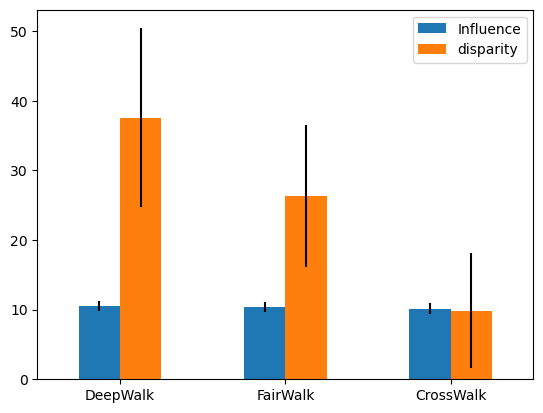
\includegraphics[width=0.45\textwidth]{images/infmax_deepwalk_synthetic3.png}}\
   \subfloat[IM -- Rice-Facebook -- DeepWalk]{
   \includegraphics[width=0.45\textwidth]{images/infmax_deepwalk_rice.png}}
   % \subfloat[IM -- Twitter -- DeepWalk]{
   % \includegraphics[width=0.45\textwidth]{images/infmax_deepwalk_twitter.png}}\
   \subfloat[IM -- Rice-Facebook -- Node2Vec]{
   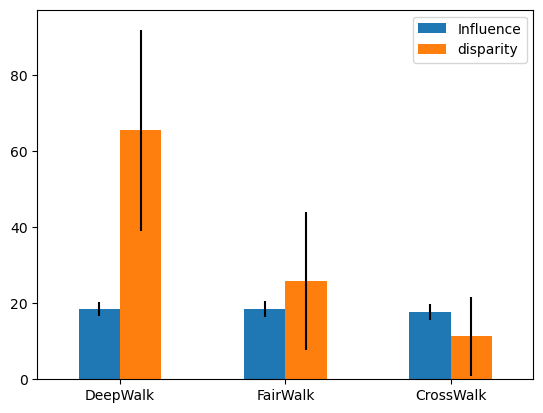
\includegraphics[width=0.45\textwidth]{images/infmax_node2vec_rice.png}}\
   \subfloat[NC -- Rice-Facebook -- DeepWalk]{
   \includegraphics[width=0.45\textwidth]{images/nodeclass_deepwalk_rice.png}}
   \subfloat[LP -- Rice-Facebook -- DeepWalk]{
   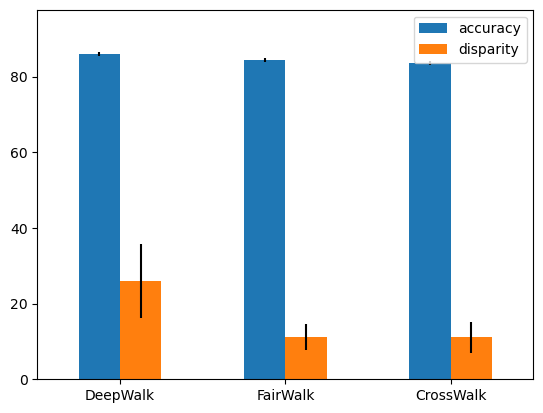
\includegraphics[width=0.45\textwidth]{images/linkpred_deepwalk_rice.png}}\
   % \subfloat[LP -- Twitter -- DeepWalk]{
   % \includegraphics[width=0.45\textwidth]{images/linkpred_deepwalk_twitter.png}}\
\caption{\textbf{Visualization of reproduction results.}}
\label{fig:visualization-results}
\end{figure}

\clearpage

\section{Results for Twitter dataset}
\label{sec:twitter-results}

\begin{table}[!htbp]
    \centering
    \resizebox{\textwidth}{!}{\begin{tabular}{llrrrr}
        \toprule
        \textbf{Task} & \textbf{Embeddings} & \multicolumn{2}{c}{\textbf{Influence/accuracy}} & \multicolumn{2}{c}{\textbf{Disparity}} \\
        & & \textbf{Original} & \textbf{Reproduced} & \textbf{Original} & \textbf{Reproduced} \\
        \midrule
           Influence maximization &  DW    & $\sim$1.37 & 1.30 (0.10) & $\sim$0.09 & \textbf{0.58 (0.45)} \\
           & FW+DW & $\sim$1.40 & 1.33 (0.09) & $\sim$0.15 & 0.54 (0.64) \\
           & CW+DW & $\sim$1.43 & 1.33 (0.10) & $\sim$0.08 & \textbf{1.22 (0.77)} \\
        \midrule
           Link prediction &  DW    & 69.45 & \textbf{92.66 (0.47)} & 83.65 & \textbf{3.47 (3.41)} \\
           & FW+DW & 69.17 & \textbf{94.65 (0.35)} & 63.82 & \textbf{5.24 (5.02)} \\
           & CW+DW & 68.02 & \textbf{94.66 (0.4)} & 42.79 & \textbf{3.93 (3.53)} \\
        \bottomrule
    \end{tabular}}
    \caption{\textbf{Reproduction results for Twitter dataset.} Comparison of original results and their reproduced counterparts. We use DeepWalk (DW) and Node2Vec (N2V) embeddings either without reweighting, with FairWalk (FW), or with CrossWalk (CW). Original results over 5 runs were gathered from the original code-base. Unavailable values (preceded by '$\sim$') were estimated from plots in the paper. Reproduced results over 50 runs are presented with standard deviations in parentheses. For original results deviating by more than one standard deviation, the reproduced results are in \textbf{bold}.}
    \label{tab:twitter-results}
\end{table}



\clearpage
\section{Other visualizations}

% \begin{figure}[!htbp]
%    \subfloat[Varying -  $walk$ $length$  ]{
%    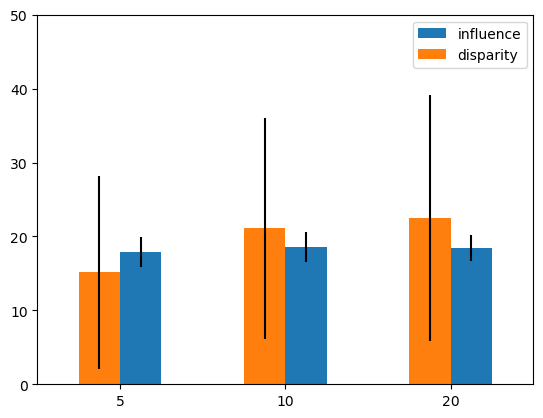
\includegraphics[width=0.49\textwidth]{images/paramsweeps/walk_length_sweep.png}}
%    \subfloat[Varying - $walks$ $per$ $node$]{
%    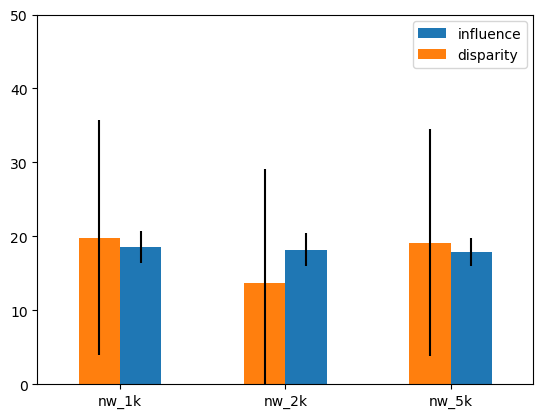
\includegraphics[width=0.49\textwidth]{images/paramsweeps/walks_per_node_sweep.png}}
% \caption{\textbf{Comparison of the Impact of $walk$ $length$ and $walks$ $per$ $node$ hyperparameters.} This was done for influence maximization on the Rice-Facebook dataset.}
% \label{fig:paramsweep2}
% \end{figure}

\begin{figure}[!htbp]
   \subfloat[Performance on Rice-Facebook dataset]{
   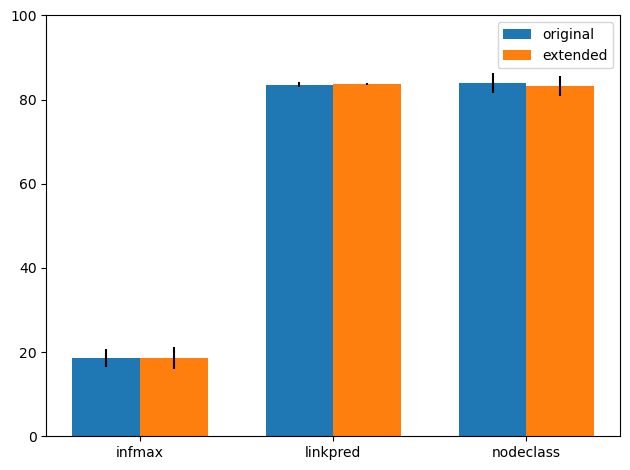
\includegraphics[width=0.49\textwidth]{images/origvstheirs_accuracies.png}}
   \subfloat[Disparity on Rice-Facebook dataset]{
   \includegraphics[width=0.49\textwidth]{images/origvstheirs_disparities.png}}
\caption{\textbf{Comparison of CrossWalk implementations in original formulation and proposed extended formulation (20 trials).} The mean of the disparity seems higher for our extended implementation, but this very likely due to the limited amount of trials and the very large standard deviations.}
\label{fig:ours-vs-theirs}
\end{figure}


\begin{figure}[!htbp]
   \subfloat[without reweighting]{
   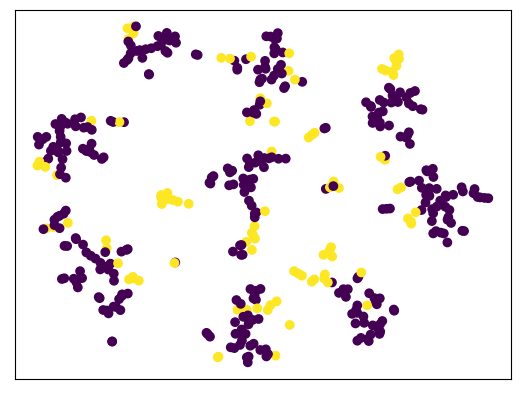
\includegraphics[width=0.49\textwidth]{images/skip_embedding.png}}
   \subfloat[with CrossWalk]{
   \includegraphics[width=0.49\textwidth]{images/crosswalk_embedding.png}}
\caption{\textbf{T-SNE visualization of DeepWalk embeddings of Rice-Facebook dataset without fairness-enhancing reweighting strategy and with CrossWalk.}
% Differences in the quality of embeddings when applying CrossWalk. showing the difference of node embeddings when CrossWalk is applied. of the effects of CrossWalk on node embeddings generated by DeepWalk of Rice-Facebook dataset.} 
Color of the nodes represents their affiliation with groups defined by the protected characteristic. In line with the authors intentions, one can observe that embeddings of nodes from different groups appear closer together after CrossWalk has been applied.}
\label{fig:visualization-embeddings}
\end{figure}